\newpage
\section{Montagne}

\begin{figure}[h]
    \centering
    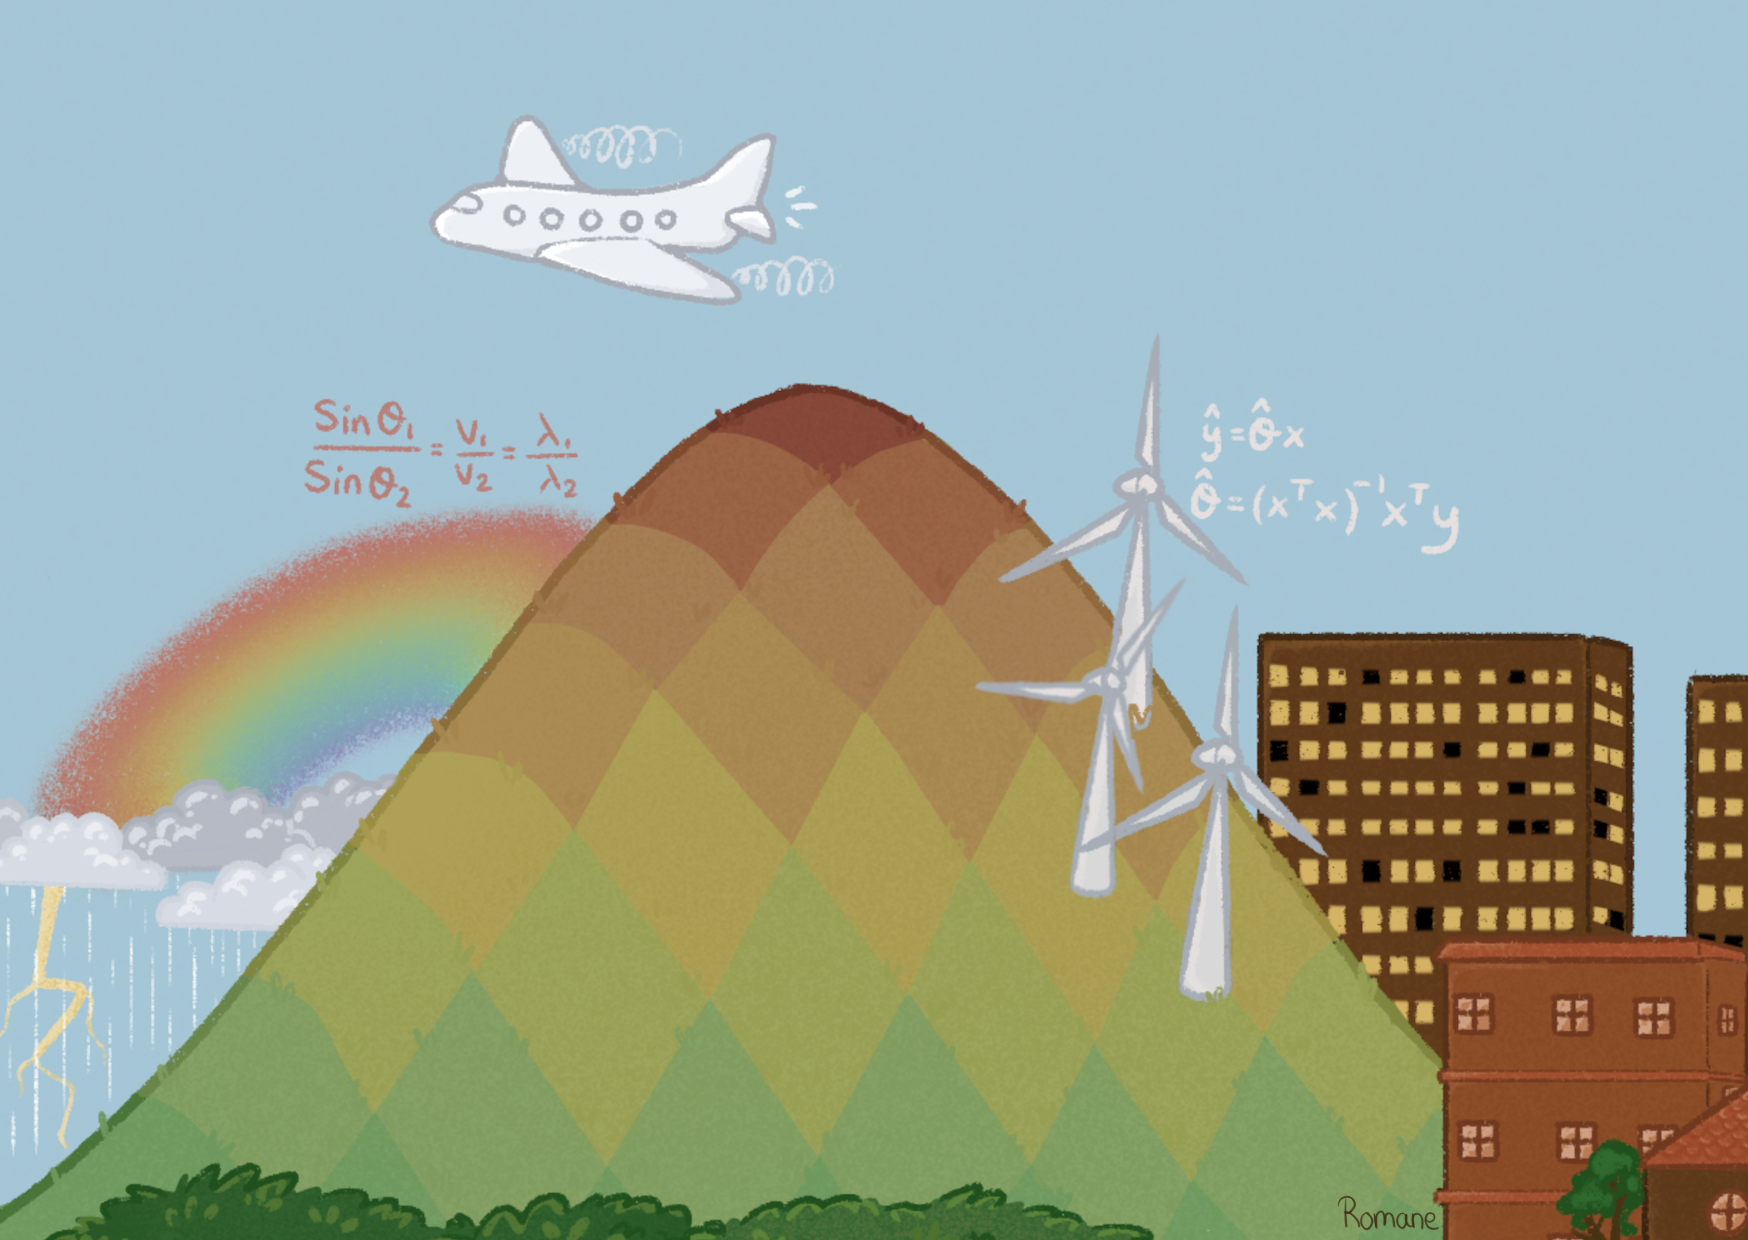
\includegraphics[height=0.5\textheight]{Cartes_postales/carte07-montagne.png}\label{fig:c07}
    \caption{Carte postale: Montagne}
\end{figure}

Sais-tu qu'on a des objets mathématiques avec des dimensions non entières? En géométrie classique, on étudie souvent des objets comme des segments, carrés, sphères ou d'autres formes simples, avec des dimensions entières, comme 1, 2 ou 3. La dimension permet de donner des précisions sur notre objet comme son périmètre et son aire. Cependant, il y a beaucoup de formes plus complexe où cette approche ne marche pas. Voici par exemple une fractale appelé la fractale de Sierpinski. On part d'un triangle équilatéral, qu'on découpe en 4 triangles équilatéraux et on retire le triangle central. Puis on recommence dans chaque triangle, indéfiniment. Avec une approche classique, on obtient une surface infini et une aire nulle en dimension 2. Donc pas très utile pour comprendre ce qui se passe.

\begin{figure}[h]
    \centering
    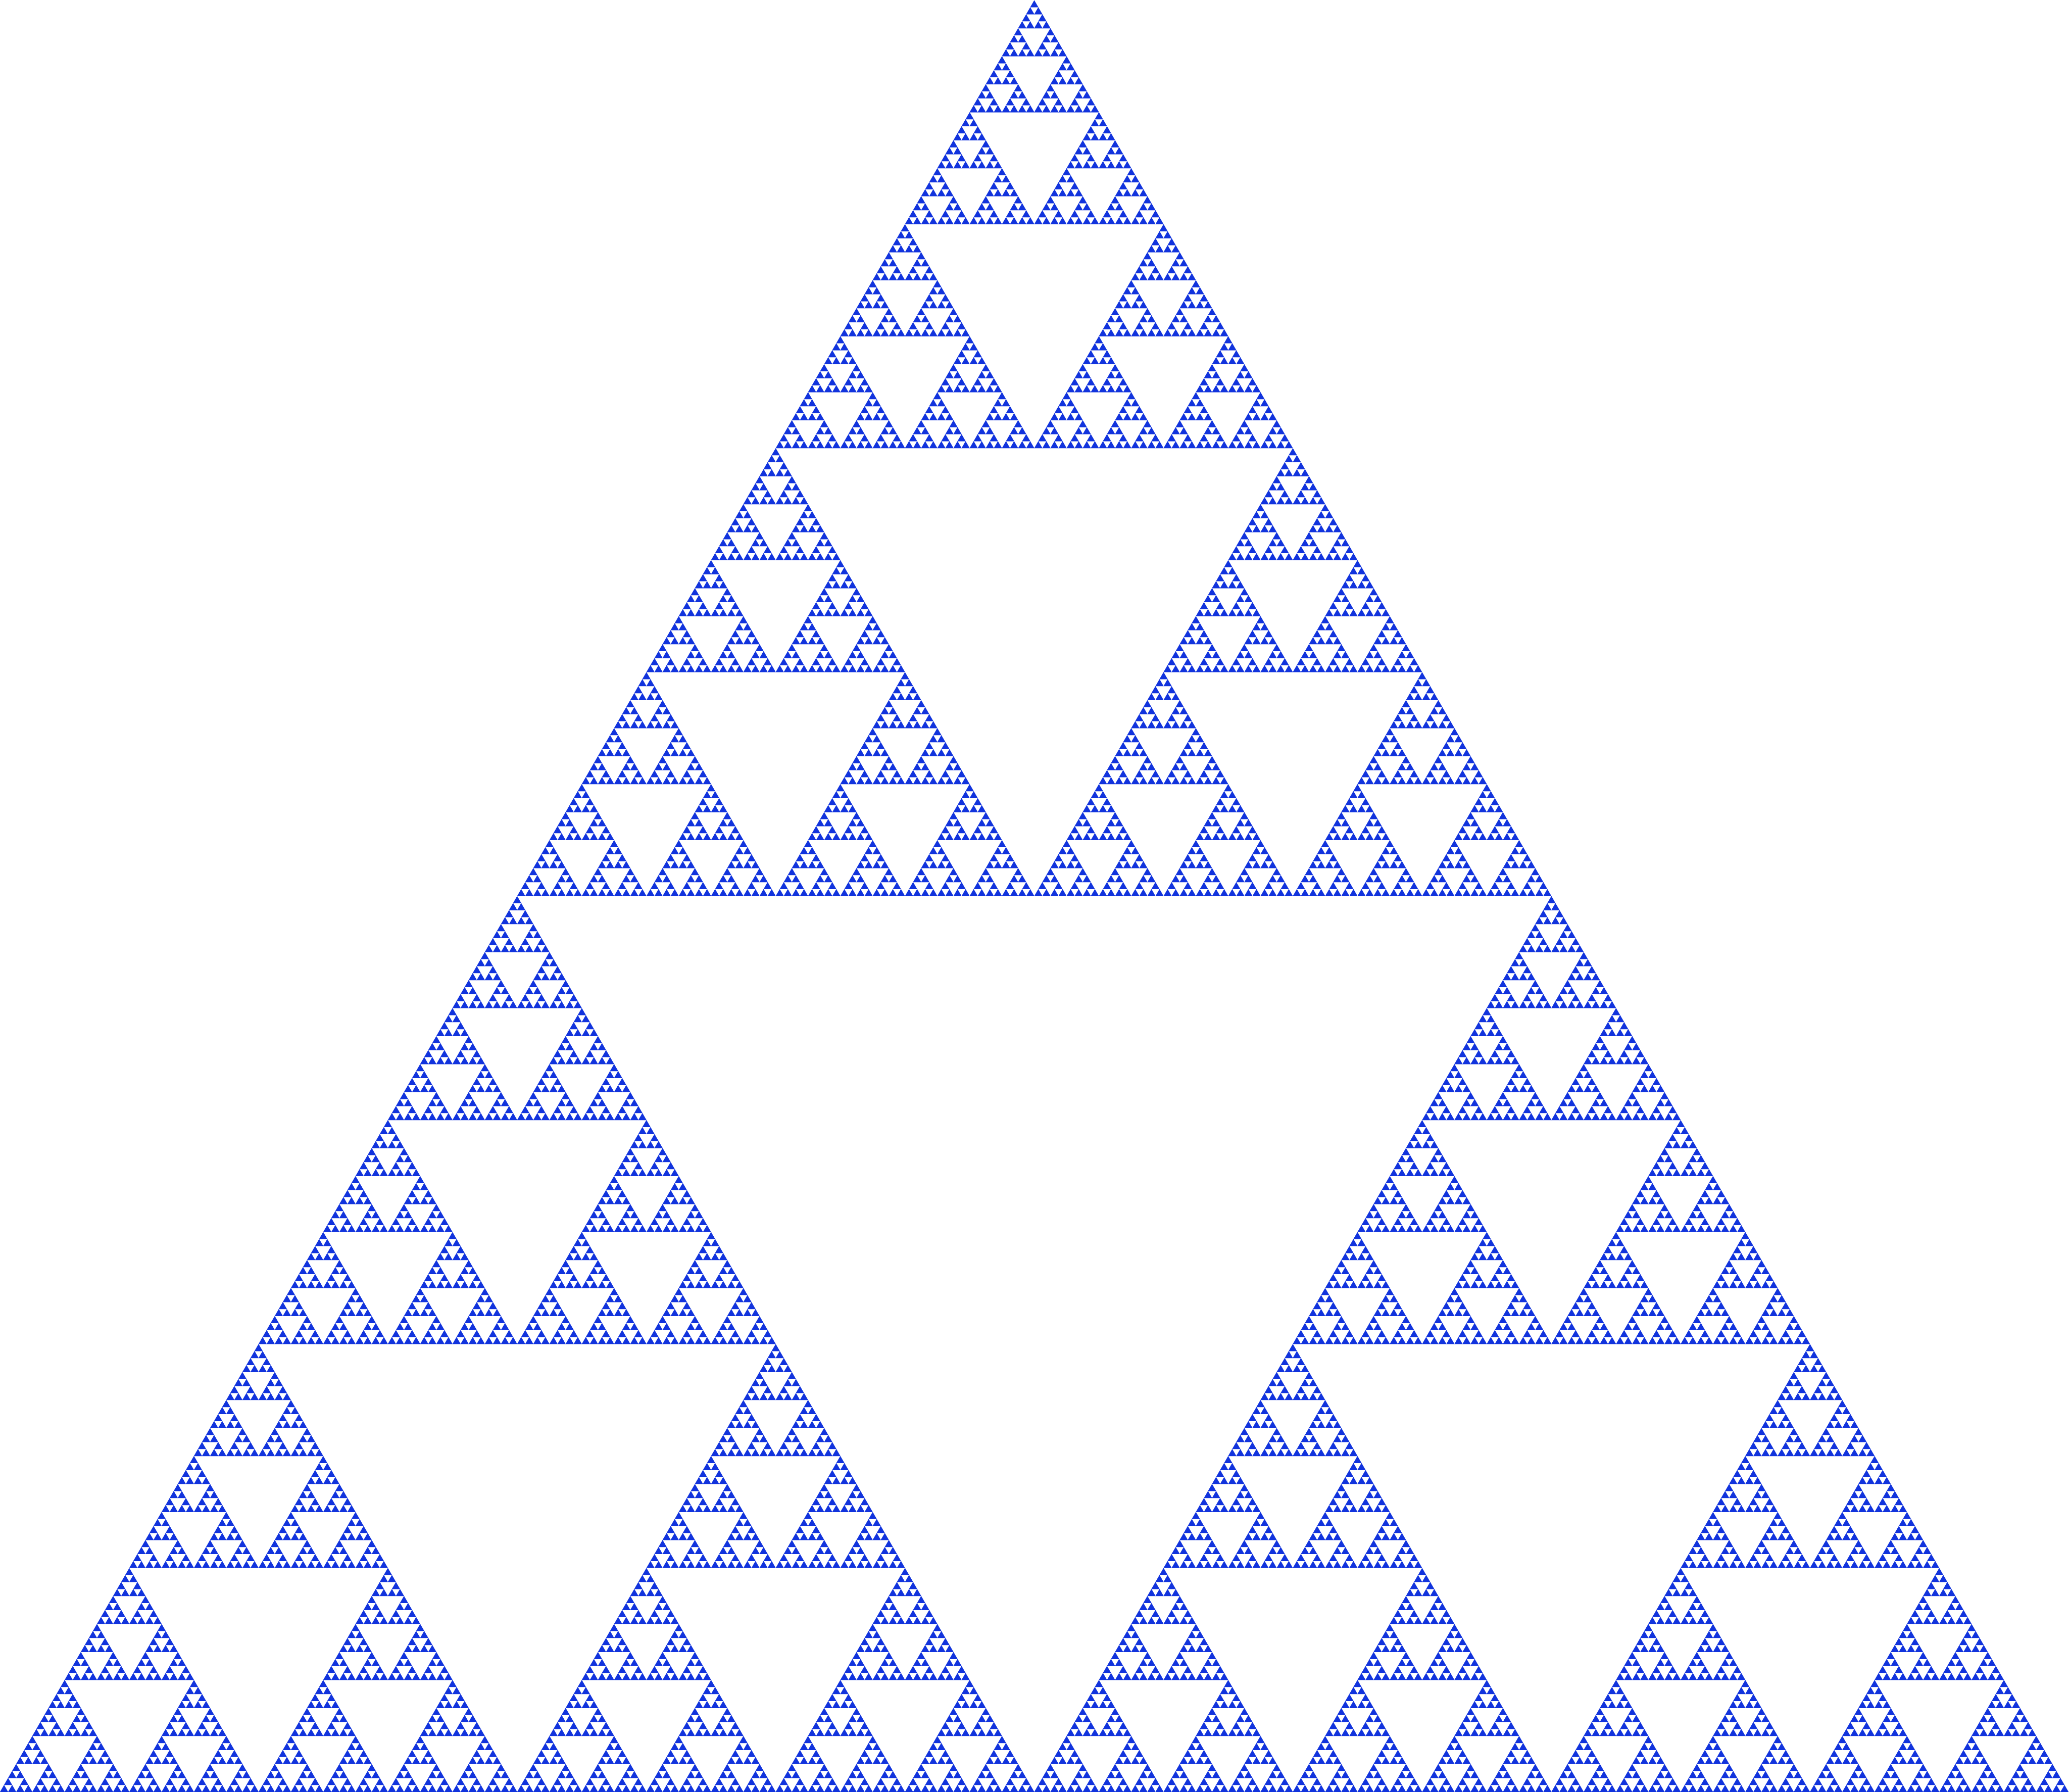
\includegraphics[height=0.1\textheight]{Images/sierpinski.png}\label{fig:c07_sierpinski}
    \caption{Le triangle de Sierpinski}
\end{figure}


En géométrie fractale, on étend cette notion de dimension, ce qui va nous donner une idée de la rugosité de notre objet. Si notre objet est très similaire à un segment, sa dimension sera proche de 1, et si il est chaotique comme la côte d'Angleterre, il aura une dimension plus grande comme 1,2. Ici, la dimension de cette fractale est d'environ 1,585. Une mer calme a une dimension fractale autour de 2,05 à 2,1 par exemple alors que la chaîne de montagnes en Himalaya, aura une dimension fractale plus proche de 2,4 ou 2,6. La dimension fractale est très importante car elle peut être utilisé dès qu'il y a des différences de comportements dans ce qu'on étudie. Elle est utilisé dans de nombreux domaines, comme en imagerie médicale pour détecter des tumeurs par exemple (car des cellules saines sont très organisées alors que des cellules cancéreuses sont plus chaotiques, et donc leur dimensions fractales sont différentes).